\newcommand{\nocontentsline}[3]{}
\newcommand{\tocless}[2]{\bgroup\let\addcontentsline=\nocontentsline#1{#2}\egroup}
\fancyhf{}
\fancyhead[LE,RO]{\nouppercase{\thepage}}
\fancyhead[LO]{\sc \nouppercase{Appendices}}
\fancyhead[RE]{\sc \nouppercase{Appendices}}

\addtocontents{toc}{\protect\setcounter{tocdepth}{ 0}}
\chapter{Supplementary materials for Chapter 2}\label{app:npscarf}
%\addtocontents{toc}{\protect\setcounter{tocdepth}{ 0}}
%\addcontentsline{toc}{chapter}{Appendix \thechapter}

\newpage

\begin{figure}[!hpt]
\centering
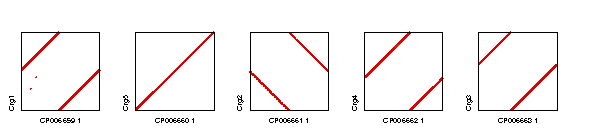
\includegraphics[width=15.84cm]{images/suppFigure1.pdf}
\caption[Alignment of the \npscarf{}'s assembly for \kp{} ATCC BAA-2146 to its reference genomes]{Alignment of the \npscarf{}'s assembly for \kp{} ATCC BAA-2146 to its draft
reference genomes (GeneBank Accession GCA\_000364385.2). The five contigs were
in complete agreement with the chromosome and four plasmids.}
\label{SF:alignKp2146}
\end{figure}

\begin{figure}[!hpt]
\centering
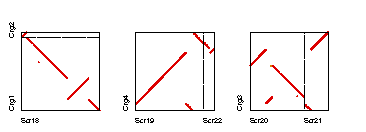
\includegraphics[width=9.76cm]{images/suppFigure2.pdf}
\caption[Alignment of the \npscarf{}'s assembly for \kp{} ATCC 13883 to its reference genomes]{Alignment of the \npscarf{}'s assembly for \kp{} ATCC 13883 to its draft
reference genomes (GeneBank Accession GCA\_000742135.1). 
For display convenience, IDs of reference sequences are abbreviated by the last two digits
before the dot in the original accession code: 
Contigs 1 and 2 were aligned to the reference Scaffold 18 (KN046818.1). 
Contig 4 was aligned to two Scaffolds 19 (KN046819.1) and
22 (KN046822.1) and Contig 3 to Scaffolds 20 (KN046820.1) and 21 (KN046821.1).}
\label{SF:alignKp13883}
\end{figure}


\begin{figure}[!hpt]
\centering
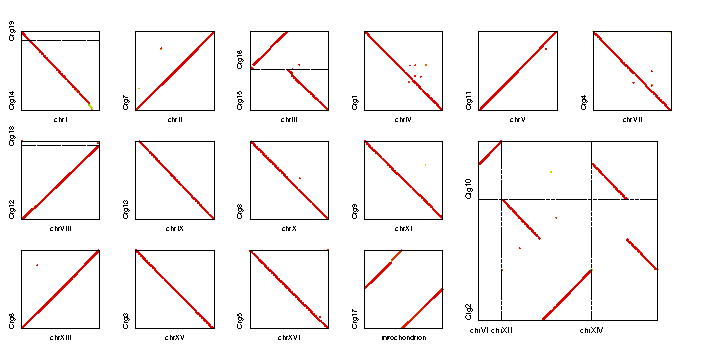
\includegraphics[width=19cm]{images/suppFigure3.pdf}
\caption[Alignment of the  \npscarf{}'s assembly for \sce{} W303 to the reference
genome of the S288C strain]{Alignment of the  \npscarf{}'s assembly for \sce{} W303 to the reference genome of the S288C strain. Ten chromosomes (II, IV, V, VII, IX, X, XI, XIII, XV, XVI and the mitochondrion) were constructed into individual contigs, three chromosomes (I, III and VIII) were into two contigs each, and three chromosomes (VI, XII and XIV) were fused into two contigs because of mis-assembly.}
\label{SF:alignW303rt}
\end{figure}


\begin{figure}[!hpt]
\centering
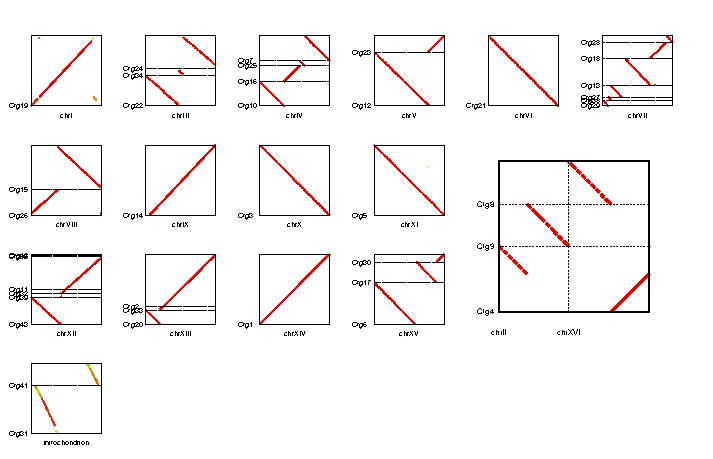
\includegraphics[width=19cm]{images/suppFigure4.pdf}
\caption[Alignment of the Canu's assembly for \sce{} W303 to the reference
genome of the S288C strain]{Alignment of the Canu's assembly for \sce{} W303 to the reference genome of the S288C strain.  Chromosomes II and XVI were fused onto three
contigs.
}
\label{SF:alignW303Canu}
\end{figure}


\begin{figure}[!hpt]
\centering
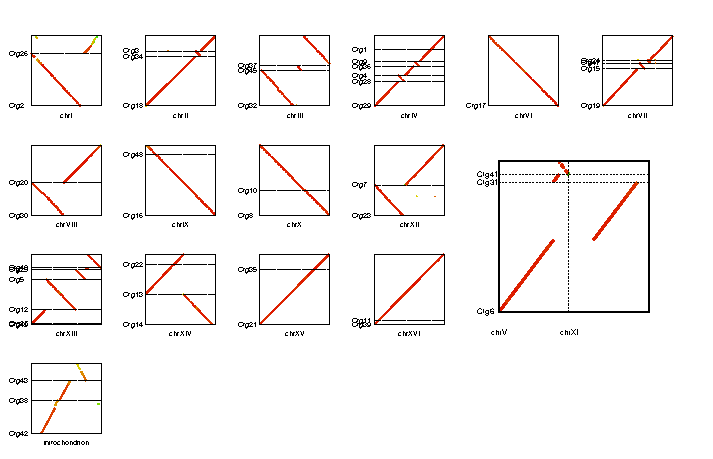
\includegraphics[width=19cm]{images/suppFigure5.pdf}
\caption[Alignment of the miniasm's assembly for \sce{} W303 to the reference
genome of the S288C strain]{Alignment of the miniasm's assembly for \sce{} W303 to the reference genome of the S288C strain. Chromosomes V and XI were fused onto three contigs.}
\label{SF:alignW303Min}
\end{figure}

\clearpage

Supplementary Table~\ref{T:mem} shows the memory usage of the tools on
the datasets described in the paper. The scaffolders (SSPACE, LINK and
\npscarf{}) were run on the short read assemblies outputed by SPAdes. We hence
only present the memory footprint from running these tools only. The memory
requirement for each pipeline should be the \emph{maximum} between memory usage
of the tool and SPAdes. For NaS and Nanocorr, the error correction steps were
distributed across hundreds of jobs, each consumed a small memory footprint. We
report here only the memory usage from running  The values reported in the table
were from running Celera Assembler. Note that we ran Celera Assembler on
differing configurations, and we reported the here the memory usage of the
configuration resulting in the most complete assembly.
Memory reported for Canu and Miniasm was the \emph{maximum} among all tasks
in the pipeline (including Pilon and BWA-MEM) because each task can be run one
at a time; However, the reported memory usage for \npscarf{} was the \emph{sum} of 
memory for running \npscarf{} and BWA-MEM.
\begin{table}[!hpt]
\centering
\caption{Memory usage (Gb) of the different tools}
\label{T:mem}
\begin{tabular}{lrrrrrrrrrr}
% \toprule
%    &       & \cthead{1}{Assembly} & \cthead{1}{\#Contigs}      & 
%    \cthead{1}{N50}  & \cthead{1}{Mis-} &  \cthead{1}{Error}  &
%    \cthead{3}{Runtimes} \\
%    & Method & \cthead{1}{size (Mb)} &\cthead{1}{($\geq500$ bp)} &
%    \cthead{1}{(Kp)} & \cthead{1}{assemblies} & \cthead{1}{(per 100 Kb)} &  
%    \cthead{3}{(CPU hrs)} \\
\toprule
 & Kp2146 & Kp13883 & E.coli K12 & ST H58 & Sc W303\\
\hline
SPAdes & 35.67 & 34.32 & 34.24 & 10.45 & 85.99 \\
 + SSPACE & 3.41 & 4.01 & 5.09 & 2.39 & 36.84 \\
 + LINK & 28.47 & 16.33 & 44.83 & 19.89 & 233.49 \\
 + \npscarf{}{} (rt) & 2.11 & 1.11 & 2.32 & 1.27 & 4.27\\
% + \nname{} (b) & 0.67 & 0.62 & 0.62 & 0.62 & 2.37 \\
NaS + CA & 8.02 & 8.10 & 9.21 & 8.23 & 83.60 \\
Nanocorr + CA & 3.76 & 3.99 & 6.91 & 1.57 & 159.91 \\
Canu + Pilon & - & 6.78 & 6.30 & - & 56.20 \\
Miniasm + Pilon & 2.99 & 6.08 & 6.04 & 1.97 & 89.51 \\
\hline
\end{tabular}
\end{table}

\addtocontents{toc}{\protect\setcounter{tocdepth}{ 0}}
\chapter{Supplementary materials for Chapter 3}\label{app:npbarcode}
%\addtocontents{toc}{\protect\setcounter{tocdepth}{ 0}}
%\addcontentsline{toc}{chapter}{Appendix \thechapter}
\newpage

\begin{figure}[!hp]
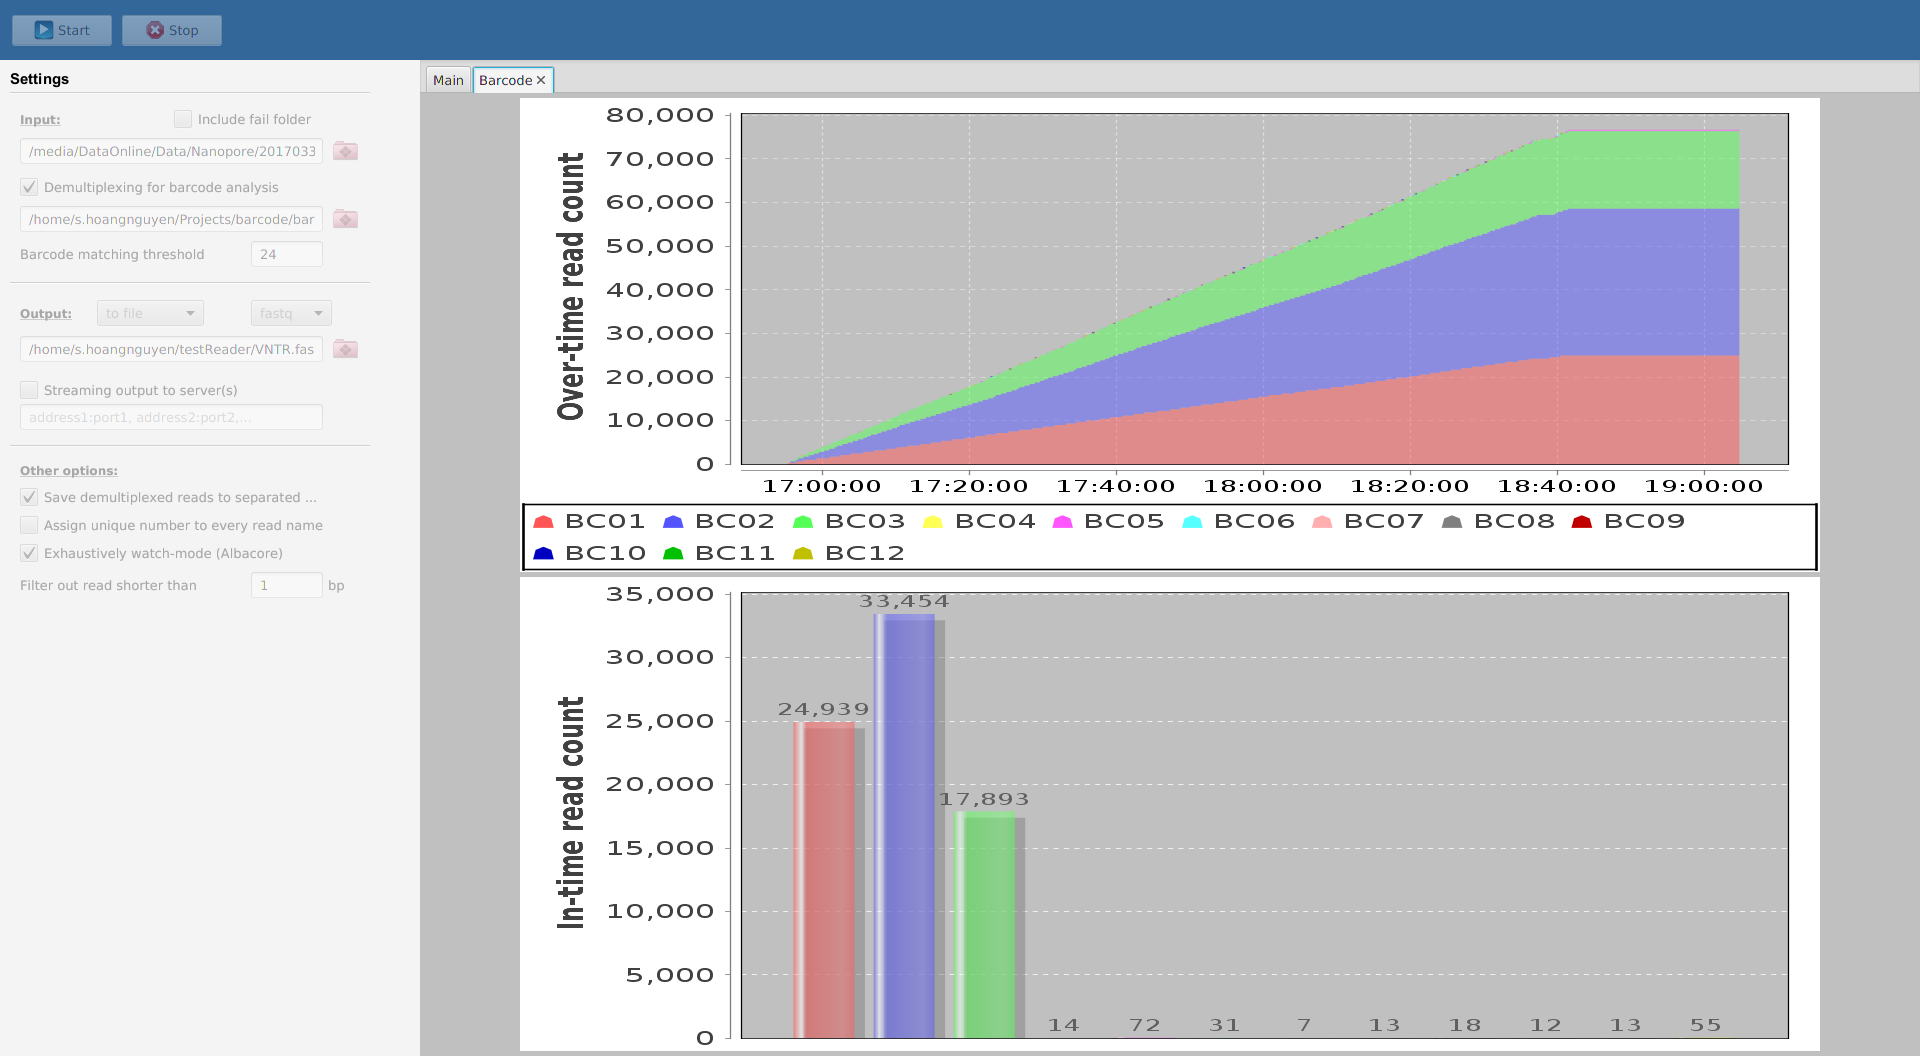
\includegraphics[width=\textwidth]{images/vntr1.png}  
\caption[PCR barcode MinION sequencing with \npbarcode{}]
{Another application of \npbarcode{} with GUI for ONT sequencing using PCR barcoding kit (3 libraries, Albacore base-caller).}
\label{supp_fig:npbarcode_pcr}
\end{figure}

\begin{table}[!htb]
\caption{Information for each of 8 samples used in the Native Barcoding sequencing protocol.}
\label{supp_tab:sample}
\centering
\begin{tabular}{l|l|l|l|r}
\textbf{ID} & \textbf{Strain}          & \textbf{Publish ID} & \textbf{Barcode ID} & \textbf{Input (ng)} \\\hline
GP\_023            & \emph{Streptococcus pneumoniae} &        ATCC 700677              & NB01                & 1,000                \\
GN\_092            & \emph{Klebsiella pneumoniae}    &         3\_GR\_13~\cite{Miranda2018}             & NB02                & 1,500                \\
GN\_093            & \emph{Acinetobacter baumannii}  &          n/a            & NB03                & 1,500                \\
GN\_096            & \emph{Klebsiella pneumoniae}    &         5\_GR\_13~\cite{Miranda2018}              & NB04                & 935                 \\
GN\_101            & \emph{Pseudomonas aeruginosa}   &          n/a            & NB05                & 1,500                \\
GN\_106            & \emph{Klebsiella pneumoniae}    &         11\_BR\_13~\cite{Miranda2018}              & NB06                & 1,500                \\
GN\_132            & \emph{Klebsiella quasipneumoniae}    &         21\_GR\_13~\cite{Miranda2018}              & NB07                & 1,000                \\
GN\_133            & \emph{Klebsiella pneumoniae}    &         22\_GR\_12~\cite{Miranda2018}              & NB08                & 1,500               
\end{tabular}
\end{table}

% From the native sequencing, we also run Porechop and poreFUME, together with Metrichor's demultiplexer for comparison. It is worth noting that since Metrichor's demultiplexer only works on 2D sequencing reads for the time we conduct the experiment, it is  therefore necessary to limit the comparison within this set.

% Each demultiplexer's output is a set of read bins where each bin is supposed to correspond to one target library. To evaluate the accuracy of the classification, we align all reads back to the references by BWA-MEM. Theoretically to be the absolute ground truth, every single read must align to exact one reference. However, this is not the case due to nanopore sequencing error rate (causing no hit found) and the similarity between 8 bacterial samples in use (causing confusions because of multiple and/or chimeric hits). 

\begin{table}[!hp]
\centering
\caption[Pairwise comparison between samples in Native Barcode Sequencing]{Pairwise comparison (using MUMmer) between 8 samples in our Native Barcode Sequencing. Value in cell $(i,j)$ is percentage (bases) of genome $i$ aligned to genome $j$. Highly identical genomes and their figures are highlighted.} 
\label{supp_tab:dnadiff}
\begin{tabular}{l|llllllll}
\hline
& GP\_023 & \textbf{GN\_092} & GN\_093 & \textbf{GN\_096} & GN\_101 & \textbf{GN\_106} & \textbf{GN\_132} & \textbf{GN\_133} \\ \hline
GP\_023 & 100 & 0.30 & 0.16 & 0.27 & 0.09 & 0.34 & 0.28 & 0.30 \\
\textbf{GN\_092} & 0.14 & 100  & 0.30 & \textbf{87.28} & 1.09 & \textbf{92.74} & \textbf{78.42} & \textbf{97.11} \\
GN\_093 & 0.13 & 0.32  & 100 & 0.32 & 0.30 & 0.25 & 0.23 & 0.3  \\
\textbf{GN\_096} & 0.14 & \textbf{88.84}  & 0.31 & 100 & 1.27 & \textbf{88.10}  & \textbf{79.75}  & \textbf{86.24}  \\
GN\_101 & 0.03 & 0.90 & 0.15 & 1.00 & 100 & 1.02 & 0.73  & 0.72 \\ \textbf{GN\_106} & 0.17  & \textbf{93.96} & 0.17 & \textbf{87.47} & 1.19  & 100 & \textbf{79.65} & \textbf{91.86}  \\
\textbf{GN\_132} & 0.13 & \textbf{79.99}  & 0.16  & \textbf{79.94} & 0.84 & \textbf{80.50} & 100 & \textbf{79.66} \\
\textbf{GN\_133} & 0.15 & \textbf{99.99} & 0.26 & \textbf{87.31} & 0.93    & \textbf{93.47} & \textbf{80.50} & 100 \\ \hline
\end{tabular}
\end{table}

% \tab{tab:dnadiff} shows the intersection of those genomes in pairs. From the table, 5 out of 8 samples shares significant identical genome's content. Especially there are three bacteria namely GN\_092, GN\_106 and GN\_133 possessing more than 90\% identity thus rooting great possibility of confusing alignments. On the other hand, 3 out of 8 genomes are  significantly unique when only sharing around 1\% or less of common bases to another. In fact, the only gram negative species GP\_23 is the most diverged isolate amongst all.

% Despite of aforementioned issues, for the comparison purpose, we can still have a decent estimation on the accuracy of the binning algorithms based on alignment. We extract the best out of all possible alignments for a read and assign its origin as the best-hit reference. Results are shown in \fig{fig:comparison}. For better illustration, divergences between samples are reflected via corresponding color palette, e.g. GN\_092, GN\_106 and GN\_133 are filled with nearly identical colors due to their highly similarity.

\begin{figure}[!hpt]
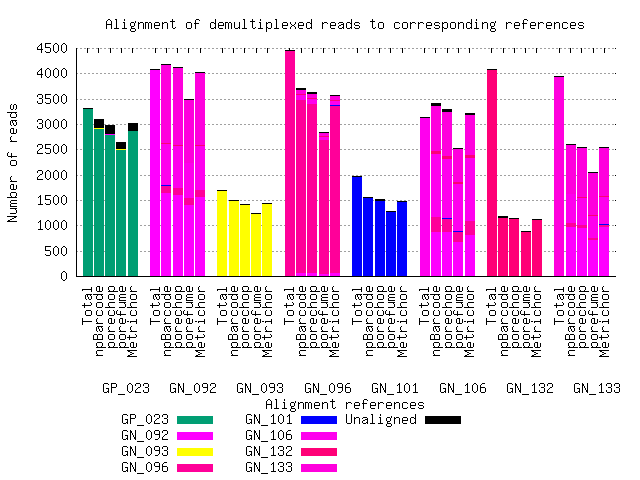
\includegraphics[width=\textwidth]{images/alignment.png}
\caption[Comparison of ONT Native Barcode Sequencing demultiplexing accuracy]
{Comparison of ONT Native Barcode Sequencing (8 libraries) demultiplexing accuracy. The bars present the number of aligned reads to references. Each group of bars correspond to a demultiplex bin. Bars in a group, from left to right, are from (1) the total data set (2) \npbarcode{} (3) Porechop (4) poreFUME demultiplex. GN\_092, GN\_106, GN\_133 together with GN\_096 and GN\_132 are very close thus being filled by similar colors (pink-red).}
\label{supp_fig:comparison}
\end{figure}

% In general, the performances of 4 demultiplexers are stably comparable, especially \npbarcode{}, Porechop and Metrichor. The number of correctly aligned reads from \npbarcode{} is slightly higher than the other two while poreFUME's figures are the lowest among all. 
% In comparison with the total number of reads aligned to the reference, the number of corresponding reads discovered by demultiplexers are considerable close except for the cases of GN\_132 and GN\_133. We suggest that this is due to artifact during library preparation and/or barcode ligation step that destroy the integrity of the barcode sequences and make them more difficult to be detected.

\begin{table}[!hpt]
\centering
\caption[Statistics for identification of GP\_023]{True Positive and True Negative rate on identification of Gram Negative species GP\_023. 

It can be seen that \npbarcode{} has the highest rate of true positive (sensitivity 88.26\%) and the lowest rate of true negative (specificity 99.19\%). 
The common behavior for all demultiplex algorithms is to takes higher/lower risk of wrong classification in exchange for the greater/lesser discovery rate possible. This ratio has to be managed in a proper way depending on different situations yet can be adjusted by parameter calibration. For this use case with default parameter set, \npbarcode, Porechop and Metrichor built-in demultiplex return comparable results while poreFUME is slightly more conservative.} 
\label{supp_tab:sensitivity}
\begin{tabular}{l|llll}
\hline
& \textbf{npBarcode} & \textbf{Porechop} & \textbf{poreFUME} & \textbf{Metrichor} \\ \hline
True Positive & 2,924 & 2,812 & 2,515 & 2,875 \\ 
True Negative & 22,125 & 22,147 & 22,177 & 22,155 \\ 
False Positive & 181 & 159 & 129 & 151 \\ 
False Negative & 389 & 501 & 798 & 438 \\ \hline
\textbf{Sensitivity (\%)} & 88.26 & 84.88 & 75.91 & 86.78 \\ 
\textbf{Specificity (\%)} & 99.19 & 99.29 & 99.42 & 99.32 \\  \hline
\end{tabular}
\end{table}

\begin{lstlisting}[float,language=bash,caption={An example of \emph{script.sh} used for \npbarcode{}, assuming that all SPAdes output folders are located in the same directory as this script and have name containing the barcoded sample.},label=lst:script]
#!/bin/bash
dirname=`find . -maxdepth 1 -type d -name "*${1}*" -print -quit`
bwa index ${dirname}/contigs.fasta
bwa mem -t 16 -k11 -W20 -r10 -A1 -B1 -O1 -E1 -L0 -a -Y -K 10000 \
	${dirname}/contigs.fasta - 2> /dev/null | \
jsa.np.npscarf -realtime -read 100 -time 1 -b - \
	-seq ${dirname}/contigs.fasta -spadesDir ${dirname} \
	-prefix ${1} > ${1}.log 2>&1
\end{lstlisting}


\begin{table}[!hpt]
\centering
\scriptsize
\caption[Real-time emulation of time to detect resistance genes from DNA sequencing]{Real-time emulation of time to detect resistance genes from DNA sequencing. \textbf{Bold} represents genes or gene family detected in final assembly and \# displays more than three genes grouped within this family. Genes displayed in order of time detected. Brackets represent class of antibiotic this gene confers resistance which includes: A, aminoglycoside; B, beta-lactam; F; fosfomycin; Fu; fusidic acid, M, macrolide; P, phenicol; Q, quinolone; R, rifampicin; S, sulphonamide; T, tetracycline; Tr, trimethoprim; V, vancomycin.}
\label{supp_tab:emulate}
\begin{tabular}{|l|c|}
\hline
{\small Time (mins)} & {\small Resistance gene(s) detected}  \\ \hline \hline
\multicolumn{2}{|c|}{\small Isolate: 1\_GR\_13 Total run time: 1279 mins} \\ \hline \hline

10          & \begin{tabular}[c]{@{}c@{}}\textbf{oqxA} (Q), \textbf{dfrA1} (Tr), \textbf{dfrA14} (Tr), \textbf{dfrA23} (Tr), \textbf{blaVIM-27}\# (B), \textbf{sul1/3} (S), \textbf{strA} (A), \\ \textbf{aph(3’)-Ia/c} (A), strB (A), aadB (A), \textbf{mph(A} (M), \textbf{blaTEM-1B}\# (B), \textbf{oqxB} (Q), \textbf{rmtB2} (A)\end{tabular}             \\ \hline
30          & \begin{tabular}[c]{@{}c@{}}sul2 (S), \textbf{ARR-2/3/6} (R), \textbf{blaOXA-10}\# (B), \textbf{blaVEB-1}\# (B), \textbf{tet(G)} (T), \textbf{cmlA1} (P), floR (P), \\ \textbf{blaSHV-11}\# (B), \textbf{fosA} (F)\end{tabular}                                                                      \\ \hline
60          & ARR-3 (R), aac(6’)Ib\# (A), ARR-7 (R), aac(2’) (A), cml (P)                                                                                                                                                                          \\ \hline
120         & aac(3’)-IIIc (A)                                                                                                                                                                                                                     \\ \hline
300         & aac(3’)-IIIb (A), aac(6’)-Ic (A),                                                                                                                                                                                                    \\ \hline
600         & blaPAO (B), aph(3’)-IIb (A), aph(6)-Ic (A)                                                                                                                                                                                           \\ \hline
900         & catpC233 (P), blaOKP (B)                                                                                                                                                                                                             \\ \hline
1200        & \textbf{tet(A)} (T)                                                                                                                                                                                                                           \\ \hline \hline
\multicolumn{2}{|c|}{\small Isolate: 2\_GR\_12 Total run time: 2468 mins}                                                                                                                                                                                                             \\ \hline \hline
10          & \textbf{blaKPC-2}\# (B), \textbf{blaTEM-1A}\#(B), \textbf{aac6Ib/-cr}\# (A), \textbf{cmlA1} (P), \textbf{dfrA12} (Tr), \textbf{sul1/ 3} (S)                                                                                                                                                \\ \hline
30          & \textbf{rmtB2} (A), \textbf{oqxA} (Q), \textbf{dfrA14} (Tr), blaPAO (B)                                                                                                                                                                                         \\ \hline
60          & \begin{tabular}[c]{@{}c@{}}\textbf{oqxB} (Q), strA (A), strB (A), \textbf{aph(3’)-1a/c} (A), \textbf{sul2} (S), \textbf{blaSHV-11/12}\# (B), \textbf{mph(A)} (M), \\ \textbf{catA1} (P), \textbf{tet(G)} (T), \textbf{blaOXA-9}\# (B), \textbf{aadA1/2}\# (A), fusB (Fu), \textbf{aac(6’)/aph(2”)} (A)\end{tabular}            \\ \hline
120         & \textbf{blaOXA-10}\# (B), floR (P), \textbf{ARR-2/3/6} (R), aadB (A), \textbf{fosA} (F), \textbf{blaVEB-1}\# (B), cml (P), \textbf{dfrA23} (Tr)                                                                                                                                   \\ \hline
300         & aac(3’)-IIIc (A), catpC233 (P), aac(3’)-IIIb (A), ARR-3 (R)                                                                                                                                                                          \\ \hline
600         & \textbf{tet(A)} (T)                                                                                                                                                                                                                           \\ \hline
900         & aph(6)-Ic (A)                                                                                                                                                                                                                        \\ \hline
1200        & -                                                                                                                                                                                                                                    \\ \hline \hline
\multicolumn{2}{|c|}{\small Isolate: 16\_GR\_13 Total run time: 1277 mins}                                                                                                                                                                                                            \\ \hline \hline
10          & blaOXA-436 (B), \textbf{sul1}/3 (S), \textbf{dfrA12} (Tr), \textbf{fosA} (F), aadB (A), strA (A), \textbf{sul2} (S), strB (A), blaCTX-M-64 (B)                                                                                                                           \\ \hline
30          & \begin{tabular}[c]{@{}c@{}}\textbf{blaOXA-48}\# (B), \textbf{aph(3’)-1a/c} (A), \textbf{mph(A)} (M), \textbf{rmtB2} (A), floR (P), \textbf{blaCTX-M-15}\# (B), \\ \textbf{aac(6’)Ib-cr}\# (A), \textbf{blaOXA-1}\# (B), \textbf{oqxB} (Q), \textbf{oqxA} (Q), \textbf{blaTEM-1B}\# (B), \textbf{blaVEB-1}\# (B), \textbf{cmlA1} (P)\end{tabular} \\ \hline
60          & \textbf{tet(G)} (T), \textbf{blaOXA-10}\# (B), \textbf{blaSHV-11}\# (B), \textbf{aac(3’)-IIa}\# (A), \textbf{ARR-2}/3/6 (R)                                                                                                                                                       \\ \hline
120         & \textbf{aadA1/2}\# (A), fusB (Fu), ermT (M), str (A), rmtG (A), \textbf{aac(6’)}/aph(2”) (A)                                                                                                                                                           \\ \hline
300         & ARR-3 (R), catpC233 (P), cml (P), aph(6)-Ic (A), aac(3’)-IIIb (A)                                                                                                                                                                    \\ \hline
600         & vanR (V), dfrA14 (Tr)                                                                                                                                                                                                                \\ \hline
900         & blaPAO (B)                                                                                                                                                                                                                           \\ \hline
1200        & aph(3’)-IIb (A)                                                                                                                                                                                                                      \\ \hline \hline
\multicolumn{2}{|c|}{\small Isolate: 20\_GR\_12 Total run time: 1277 mins}                                                                                                                                                                                                            \\ \hline \hline
10          & \textbf{aac(6’)Ib/-cr}\# (A), \textbf{blaTEM-1A}\# (B), \textbf{dfrA14} (Tr), \textbf{sul2} (S), strB (A), \textbf{blaKPC-2}\# (B),\textbf{ tet(A)} (T)                                                                                                                                    \\ \hline
30          & \textbf{oqxA} (Q), \textbf{blaSHV-11/12}\# (B), \textbf{aph(3’)-Ia} (A), \textbf{fosA} (F), \textbf{blaOXA-9} (B), \textbf{oqxB} (Q), aph(6)-Ic (A)                                                                                                                                        \\ \hline
60          & -                                                                                                                                                                                                                                    \\ \hline
120         & aac(2’) (A), catpC233 (P), aac(3’)-IIIb (A)                                                                                                                                                                                          \\ \hline
300         & ermT (M), blaPAO (B),\textbf{ aac(6’)}/aph(2”) (A), catpC221 (P)                                                                                                                                                                              \\ \hline
600         & rmtf (A), ermG (M)                                                                                                                                                                                                                   \\ \hline
900         & aac(3’)-IIIc (A), aac(6’)-Ic (A)                                                                                                                                                                                                     \\ \hline
1200        & vatB (M), ARR-2/3/6 (R), aadB (A)                                                                                                                                                                                                    \\ \hline
\end{tabular}
\end{table}

\addtocontents{toc}{\protect\setcounter{tocdepth}{ 0}}
\chapter{Supplementary materials for Chapter 4}\label{app:npgraph}
%\addtocontents{toc}{\protect\setcounter{tocdepth}{ 0}}
%\addcontentsline{toc}{chapter}{Appendix \thechapter}
\newpage

\begin{longtable}[!hpt]{llcrrrrr}
\toprule
    &       & Assembly & \#Contigs  & N50  & Mis- &  Mismatch & Indel \\
    & Method & size (bp) &($\geq500$ bp) & (bp) & assemblies & (per 100 Kb) & (per 100 Kb) \\
\hline  
\rowcolor{Gray}
 \multicolumn{8}{l}{ random sequences no repeats: good} \\ %
\hline
\rowcolor{Gray}
 & npGraph & 4080156  &  2  &  3990078  &  0  & 0  & 0\\
\rowcolor{Gray}
 & npScarf & 4110000  &  3  &  4000000  &  0  &  0 & 0\\
\rowcolor{Gray}
& Unicycler & 4110000  &  3  &  4000000  &  0  &  0 &  0\\
\hline
 \multicolumn{8}{l}{ random sequences no repeats: medium} \\ %
\hline
 & npGraph & 4080112  &  2  &  3990056  & 0   &  0  & 0\\
 & npScarf & 4110000  &  3  &  4000000  &  0  &  0 & 0\\
 & Unicycler & 4110000  &  3  &  4000000  &  0  &  0 &  0\\
\hline
\hline  
\rowcolor{Gray}
 \multicolumn{8}{l}{ random sequences some repeats: good} \\ %
\hline
\rowcolor{Gray}
 & npGraph & 4107894  &  3  &   3997894 &  0  & 0.05  & 0.07\\
\rowcolor{Gray}
 & npScarf & 4109612  &  3  &  4001483  &  0  & 0  & 1.27\\
\rowcolor{Gray}
& Unicycler & 4110000  &  3  &  4000000  &  0  &  0 &  0\\
\hline
 \multicolumn{8}{l}{ random sequences some repeats: medium} \\ %
\hline
 & npGraph & 4107652  &  3  &  3997652  &  0 &  0 & 0\\
 & npScarf & 4105026  &  3  &  3999803  &  0  & 0.02  & 1.22\\
& Unicycler & 4110000  &  3  &  4000000  &  0  &  0 &  0\\
\hline
\hline  
\rowcolor{Gray}
 \multicolumn{8}{l}{ random sequences many repeats: good} \\ %
\hline
\rowcolor{Gray}
 & npGraph & 4099244  &  8  &  3978164  &  1  &  0.39 & 0.15\\
\rowcolor{Gray}
 & npScarf & 4287145  &  9  &  3951858  &  20  & 0.95  & 6.49\\
\rowcolor{Gray}
& Unicycler & 4110013  &  3  &  4000000  &  0  &  0.1 &  0.07\\
\hline
 \multicolumn{8}{l}{ random sequences many repeats: medium} \\ %
\hline
 & npGraph & 4105107  &  9  &  2650240  &  2  &  0.37 & 0.24\\
 & npScarf & 4338709  & 10   &  3977368  &  39  & 31.88  & 64.5\\
& Unicycler & 4110012  &  3  &  4000000  &  0  &  0.22 &  0.05\\
\hline
\hline  
\rowcolor{Gray}
 \multicolumn{8}{l}{ \emph{Acinetobacter} AB30: good} \\ %
\hline
\rowcolor{Gray}
 & npGraph & 4248501  &  28  &  1176621  &  7  &  12.08 & 1.00\\
\rowcolor{Gray}
 & npScarf & 4556380  &  10  &  4293616  &  25  & 34.81  & 54.48\\
\rowcolor{Gray}
& Unicycler & 4335781  &  1  &  4335781  &  0  & 3.25  & 0.23 \\
\hline
 \multicolumn{8}{l}{ \emph{Acinetobacter} AB30: medium} \\ %
\hline
 & npGraph & 4300851  &  35  &  1052167  &  8  &  19.49 & 1.71\\
 & npScarf & 722555  &  7  &  593850  &  7  & 72.45  & 78.27\\
& Unicycler & 4352173  &  5  &  4346003  &  0  & 3.07  & 0.53 \\
\hline
\hline  
\rowcolor{Gray}
 \multicolumn{8}{l}{ \ec{} K12 MG1655: good} \\ %
\hline
\rowcolor{Gray}
 & npGraph &  4637816 &  2  &  4630090  &  3  & 6.07  & 1.30\\
\rowcolor{Gray}
 & npScarf & 4662306  &  6  &  4612921  &  30  & 12.29  & 13.16\\
\rowcolor{Gray}
& Unicycler & 4641877  &  1  &  4641538  &  1  & 1.57  & 0.17\\
\hline
 \multicolumn{8}{l}{ \ec{} K12 MG1655: medium} \\ %
\hline
 & npGraph & 4636279  &  11  &  2952199  &  2  & 9.00  & 1.49\\
 & npScarf & 4645214  &  2  &  4632777  &  20  & 24.70  & 31.24\\
& Unicycler & 4641651  &  1  &  4641651  &  0  & 2.07  & 0.15\\
\hline
\hline  
\rowcolor{Gray}
 \multicolumn{8}{l}{ \ec{} O25b H4 ST131: good} \\ %
\hline
\rowcolor{Gray}
 & npGraph & 5225953 &  20  &  1332357  &  9  & 9.46  & 1.54\\
\rowcolor{Gray}
 & npScarf &  5274462 &  8  &  5079199  &  23  &  17.58 & 5.16\\
\rowcolor{Gray}
& Unicycler & 5249446  & 3   &  5109764  &  0  &  1.56 & 0.19\\
\hline
 \multicolumn{8}{l}{ \ec{} O25b H4 ST131: medium} \\ %
\hline
 & npGraph &  5234376 &  19  &  2784386  &  4  & 13.38  & 1.50\\
 & npScarf & 5348539  &  9  &  5087364  &  30  & 27.04  & 29.95\\
& Unicycler &  5249306 & 3  &  5109624  &  1  &  1.92 & 0.29\\
\hline
\hline  
\rowcolor{Gray}
 \multicolumn{8}{l}{ \kp{} 30660 NJST258\_1: good} \\ %
\hline
\rowcolor{Gray}
 & npGraph &  5243363 &  27  &  2670458  &  6  &  9.14 & 1.56\\
\rowcolor{Gray}
 & npScarf & 5713200  &  9  &  5260757  &  30  & 8.91  &  10.78\\
\rowcolor{Gray}
& Unicycler &  5540922 &  6  &  5263221  &  0  &  0.4 & 0.29\\
\hline
 \multicolumn{8}{l}{ \kp{} 30660 NJST258\_1: medium} \\ %
\hline
 & npGraph & 5431315  &  34  &  1390117  &  5  & 5.73  & 1.32\\
 & npScarf & 5544956  &  7  &  5249381  &  23  & 5.79  & 2.99\\
& Unicycler & 5540904  &  8  &  5263203  &  2  & 4.91  & 0.43\\
\hline
\hline  
\rowcolor{Gray}
 \multicolumn{8}{l}{ \kp{} MGH 78578: good} \\ %
\hline
\rowcolor{Gray}
 & npGraph & 5398854  &  40  &  1679207  &  2  &  8.29 & 0.82\\
\rowcolor{Gray}
 & npScarf &  5700968 &  6  &  5311550  &  41  & 16.53  & 9.32\\
\rowcolor{Gray}
& Unicycler & 5694731  &  6  & 5314956   &  1  & 2.88  & 0.16\\
\hline
 \multicolumn{8}{l}{ \kp{} MGH 78578: medium} \\ %
\hline
 & npGraph &  5598574 &  28  & 5208660   &  2  &  13.5 & 1.45\\
 & npScarf & 5399020  &  3  &  5298987  &  18  & 17.37  & 8.24\\
& Unicycler & 5694811  &  6  & 5315026   &  0  &  5.76 & 0.35\\
\hline
\hline  
\rowcolor{Gray}
 \multicolumn{8}{l}{ \kp{} NTUH K2044: good} \\ %
\hline
\rowcolor{Gray}
 & npGraph & 5175218  &  13  &  2611401  &  5  &  7.68 & 0.87\\
\rowcolor{Gray}
 & npScarf & 5469248  &  3  &  5239960  &  17  &  7.07 & 1.76\\
\rowcolor{Gray}
& Unicycler & 5472694  &  2  &  5248542  &  0  & 1.32  & 0.2\\
\hline
 \multicolumn{8}{l}{ \kp{} NTUH K2044: medium} \\ %
\hline
 & npGraph & 5393198  &  16  &  1811833  &  5  & 9.36  & 1.69\\
 & npScarf &  5479301 &  3  &  5239455  &  19  &  11.31 & 4.28 \\
& Unicycler &  5472418 &  2  &  5248274  &  2  &  1.63 & 0.11 \\
\hline
\hline  
\rowcolor{Gray}
 \multicolumn{8}{l}{ \emph{Mycobacterium tuberculosis} H37Rv: good} \\ %
\hline
\rowcolor{Gray}
 & npGraph &  4309462 &  3  &  4217195  &   5 & 3.95  & 1.56\\
\rowcolor{Gray}
 & npScarf & 4539068  &  7  &  4400303  &  40  & 15.78  & 21.73\\
\rowcolor{Gray}
& Unicycler &  4411534 & 1  &  4411534  &  1  & 0.63  & 0.11\\
\hline
 \multicolumn{8}{l}{ \emph{Mycobacterium tuberculosis} H37Rv: medium} \\ %
\hline
 & npGraph & 4389387  &  7  &  4384829  &  9  & 5.75  & 1.46\\
 & npScarf &  4422649 &  3  &  4388188  &  36  &  6.87 & 3.70\\
& Unicycler & 4411372  &  1  &  4411372  &  2  & 1.41  & 0.25\\
\hline
\caption{Benchmarking \npgraph{} against \npscarf{} and Unicycler version 0.4.6}
\label{tab:benchmarking}
\end{longtable}

\addtocontents{toc}{\protect\setcounter{tocdepth}{ 0}}
\chapter{Supplementary materials for Chapter 5}\label{app:concatemer}
%\addtocontents{toc}{\protect\setcounter{tocdepth}{ 0}}
%\addcontentsline{toc}{chapter}{Appendix \thechapter}
\newpage

\begin{figure}[!ht]
\centerline{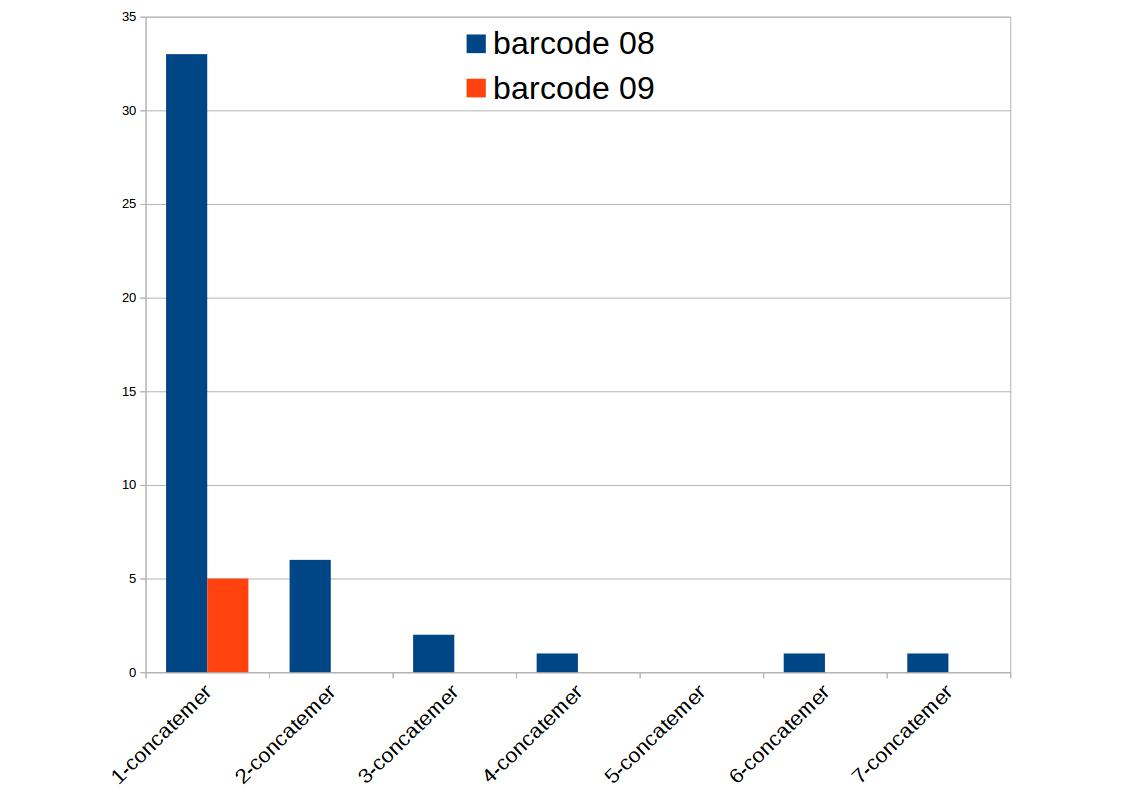
\includegraphics[width=0.9\textwidth]{images/concat_count.jpg}}
\caption[Concatemer reads count]{Number of $k$-concatemers for each sample barcode 08 and 09. $k=1\dots 7$}
\label{supp_fig:concat_count}
\end{figure}

\begin{figure}[!ht]
\centering
\subfloat[ACF for a monomer read]{
	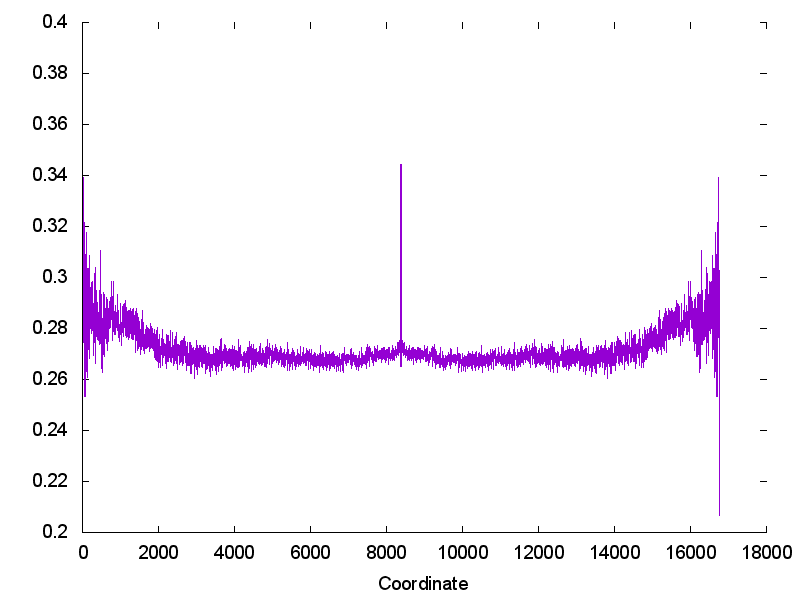
\includegraphics[width=.5\textwidth]{images/concatemer-1_std.png}
}
~
\subfloat[ACF for a 2-concatemers read]{
	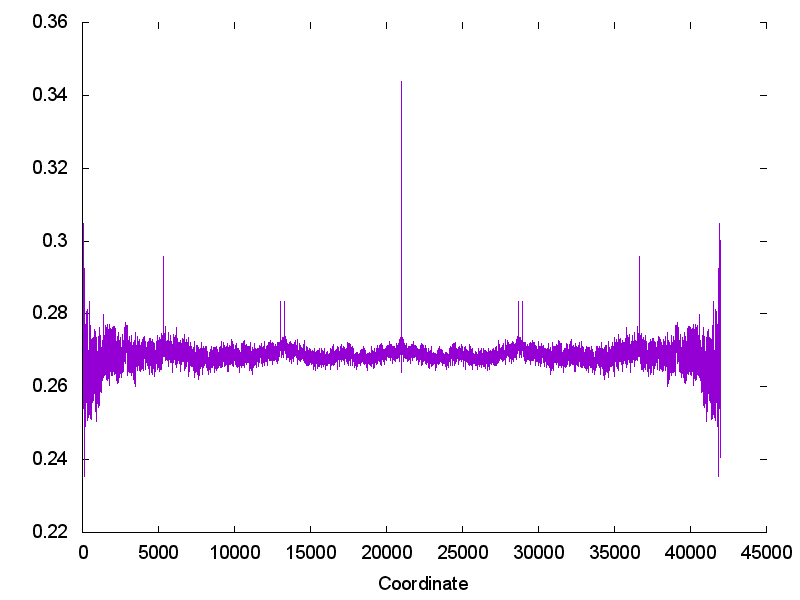
\includegraphics[width=.5\textwidth]{images/concatemer-2_std.png}
}
\\
\subfloat[ACF for a 3-concatemers read]{
	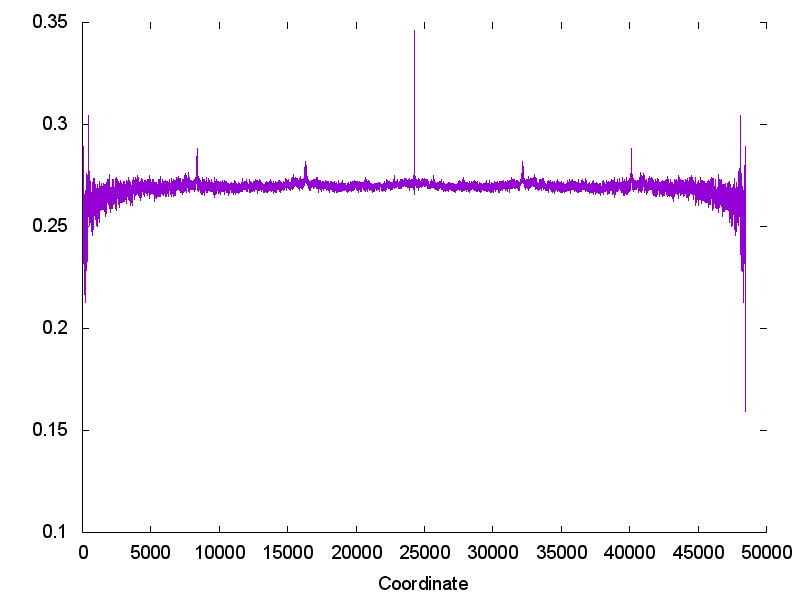
\includegraphics[width=.5\textwidth]{images/concatemer-3_std.png}
}
~
\subfloat[ACF for a 6-concatemers read]{
	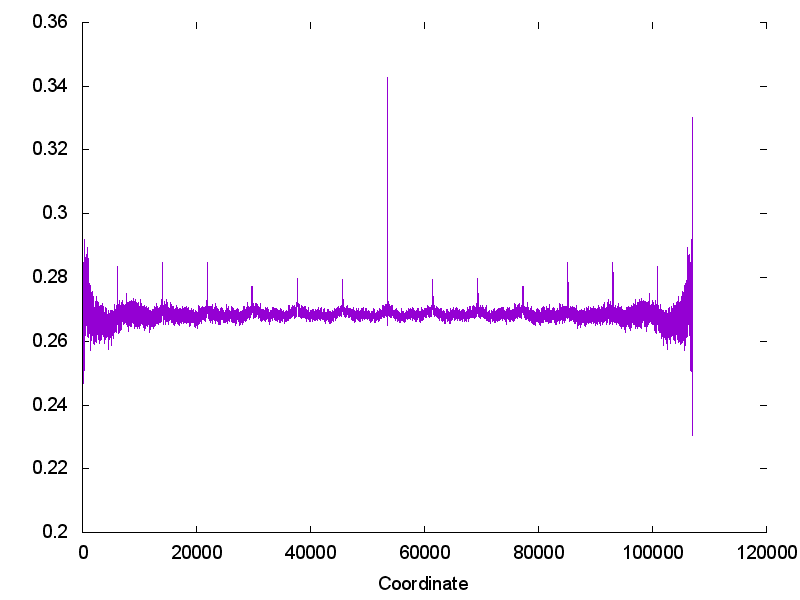
\includegraphics[width=.5\textwidth]{images/concatemer-6_std.png}
}
\\
\subfloat[ACF for the 7-concatemer read]{
	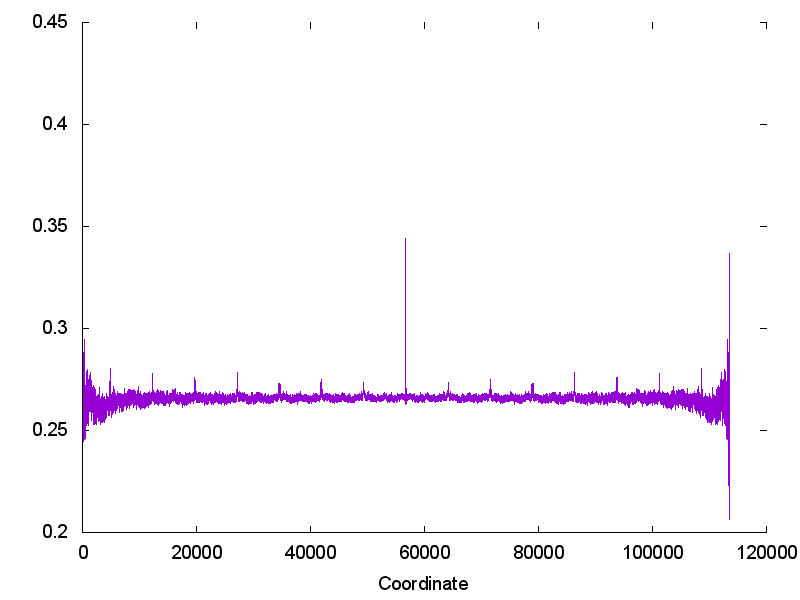
\includegraphics[width=.5\textwidth]{images/concatemer-7_std.png}
}
~
\subfloat[ACF for a random DNA sequence]{
	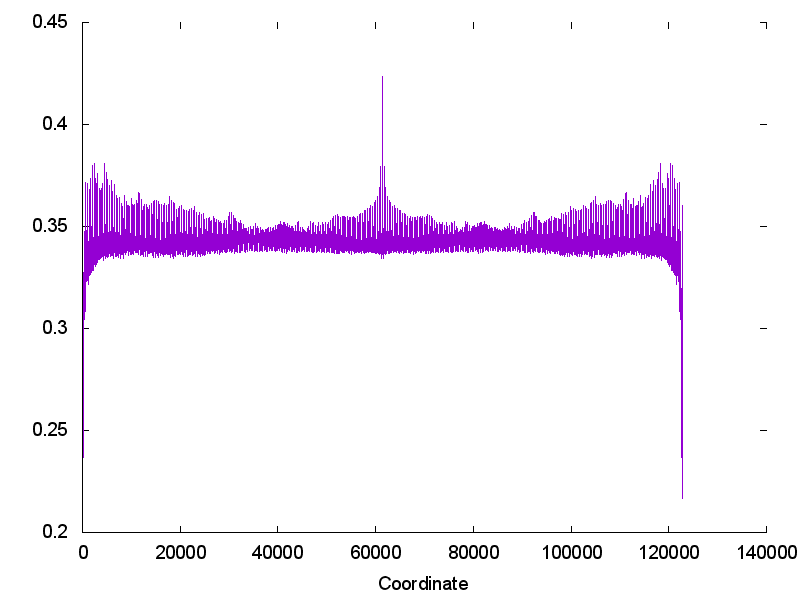
\includegraphics[width=.5\textwidth]{images/concatemer-random_std.png}
}

\caption{ACF values for a random synthetic read and several k-concatemers nanopore read detected in \emph{Cauliflower mosaic} sample (barcode 08).}
\label{supp_fig:concat_acf_dna}
\end{figure}
